\documentclass[journal,12pt,twocolumn]{IEEEtran}
\usepackage{setspace}
\usepackage{gensymb}
\usepackage{caption}
%\usepackage{multirow}
%\usepackage{multicolumn}
%\usepackage{subcaption}
%\doublespacing
\singlespacing
\usepackage{csvsimple}
\usepackage{amsmath}
\usepackage{multicol}
%\usepackage{enumerate}
\usepackage{amssymb}
%\usepackage{graphicx}
\usepackage{newfloat}
%\usepackage{syntax}
\usepackage{listings}
\usepackage{iithtlc}
\usepackage{color}
\usepackage{tikz}
\usetikzlibrary{shapes,arrows}



%\usepackage{graphicx}
%\usepackage{amssymb}
%\usepackage{relsize}
%\usepackage[cmex10]{amsmath}
%\usepackage{mathtools}
%\usepackage{amsthm}
%\interdisplaylinepenalty=2500
%\savesymbol{iint}
%\usepackage{txfonts}
%\restoresymbol{TXF}{iint}
%\usepackage{wasysym}
\usepackage{amsthm}
\usepackage{mathrsfs}
\usepackage{txfonts}
\usepackage{stfloats}
\usepackage{cite}
\usepackage{cases}
\usepackage{mathtools}
\usepackage{caption}
\usepackage{enumerate}	
\usepackage{enumitem}
\usepackage{amsmath}
%\usepackage{xtab}
\usepackage{longtable}
\usepackage{multirow}
%\usepackage{algorithm}
%\usepackage{algpseudocode}
\usepackage{enumitem}
\usepackage{mathtools}
\usepackage{hyperref}
%\usepackage[framemethod=tikz]{mdframed}
\usepackage{listings}
    %\usepackage[latin1]{inputenc}                                 %%
    \usepackage{color}                                            %%
    \usepackage{array}                                            %%
    \usepackage{longtable}                                        %%
    \usepackage{calc}                                             %%
    \usepackage{multirow}                                         %%
    \usepackage{hhline}                                           %%
    \usepackage{ifthen}                                           %%
  %optionally (for landscape tables embedded in another document): %%
    \usepackage{lscape}     


\usepackage{url}
\def\UrlBreaks{\do\/\do-}


%\usepackage{stmaryrd}


%\usepackage{wasysym}
%\newcounter{MYtempeqncnt}
\DeclareMathOperator*{\Res}{Res}
%\renewcommand{\baselinestretch}{2}
\renewcommand\thesection{\arabic{section}}
\renewcommand\thesubsection{\thesection.\arabic{subsection}}
\renewcommand\thesubsubsection{\thesubsection.\arabic{subsubsection}}

\renewcommand\thesectiondis{\arabic{section}}
\renewcommand\thesubsectiondis{\thesectiondis.\arabic{subsection}}
\renewcommand\thesubsubsectiondis{\thesubsectiondis.\arabic{subsubsection}}

% correct bad hyphenation here
\hyphenation{op-tical net-works semi-conduc-tor}

%\lstset{
%language=C,
%frame=single, 
%breaklines=true
%}

%\lstset{
	%%basicstyle=\small\ttfamily\bfseries,
	%%numberstyle=\small\ttfamily,
	%language=Octave,
	%backgroundcolor=\color{white},
	%%frame=single,
	%%keywordstyle=\bfseries,
	%%breaklines=true,
	%%showstringspaces=false,
	%%xleftmargin=-10mm,
	%%aboveskip=-1mm,
	%%belowskip=0mm
%}

%\surroundwithmdframed[width=\columnwidth]{lstlisting}
\def\inputGnumericTable{}                                 %%
\lstset{
%language=C,
frame=single, 
breaklines=true,
columns=fullflexible
}
 

\begin{document}
%
\tikzstyle{block} = [rectangle, draw,
    text width=3em, text centered, minimum height=3em]
\tikzstyle{sum} = [draw, circle, node distance=3cm]
\tikzstyle{input} = [coordinate]
\tikzstyle{output} = [coordinate]
\tikzstyle{pinstyle} = [pin edge={to-,thin,black}]

\theoremstyle{definition}
\newtheorem{theorem}{Theorem}[section]
\newtheorem{problem}{Problem}
\newtheorem{proposition}{Proposition}[section]
\newtheorem{lemma}{Lemma}[section]
\newtheorem{corollary}[theorem]{Corollary}
\newtheorem{example}{Example}[section]
\newtheorem{definition}{Definition}[section]
%\newtheorem{algorithm}{Algorithm}[section]
%\newtheorem{cor}{Corollary}
\newcommand{\BEQA}{\begin{eqnarray}}
\newcommand{\EEQA}{\end{eqnarray}}
\newcommand{\define}{\stackrel{\triangle}{=}}

\bibliographystyle{IEEEtran}
%\bibliographystyle{ieeetr}

\providecommand{\nCr}[2]{\,^{#1}C_{#2}} % nCr
\providecommand{\nPr}[2]{\,^{#1}P_{#2}} % nPr
\providecommand{\mbf}{\mathbf}
\providecommand{\pr}[1]{\ensuremath{\Pr\left(#1\right)}}
\providecommand{\qfunc}[1]{\ensuremath{Q\left(#1\right)}}
\providecommand{\sbrak}[1]{\ensuremath{{}\left[#1\right]}}
\providecommand{\lsbrak}[1]{\ensuremath{{}\left[#1\right.}}
\providecommand{\rsbrak}[1]{\ensuremath{{}\left.#1\right]}}
\providecommand{\brak}[1]{\ensuremath{\left(#1\right)}}
\providecommand{\lbrak}[1]{\ensuremath{\left(#1\right.}}
\providecommand{\rbrak}[1]{\ensuremath{\left.#1\right)}}
\providecommand{\cbrak}[1]{\ensuremath{\left\{#1\right\}}}
\providecommand{\lcbrak}[1]{\ensuremath{\left\{#1\right.}}
\providecommand{\rcbrak}[1]{\ensuremath{\left.#1\right\}}}
\theoremstyle{remark}
\newtheorem{rem}{Remark}
\newcommand{\sgn}{\mathop{\mathrm{sgn}}}
\providecommand{\abs}[1]{\left\vert#1\right\vert}
\providecommand{\res}[1]{\Res\displaylimits_{#1}} 
\providecommand{\norm}[1]{\lVert#1\rVert}
\providecommand{\mtx}[1]{\mathbf{#1}}
\providecommand{\mean}[1]{E\left[ #1 \right]}
\providecommand{\fourier}{\overset{\mathcal{F}}{ \rightleftharpoons}}
%\providecommand{\hilbert}{\overset{\mathcal{H}}{ \rightleftharpoons}}
\providecommand{\system}{\overset{\mathcal{H}}{ \longleftrightarrow}}
	%\newcommand{\solution}[2]{\textbf{Solution:}{#1}}
\newcommand{\solution}{\noindent \textbf{Solution: }}
\newcommand{\myvec}[1]{\ensuremath{\begin{pmatrix}#1\end{pmatrix}}}
\providecommand{\dec}[2]{\ensuremath{\overset{#1}{\underset{#2}{\gtrless}}}}
\DeclarePairedDelimiter{\ceil}{\lceil}{\rceil}
%\numberwithin{equation}{subsection}
%\numberwithin{equation}{section}
%\numberwithin{problem}{subsection}
%\numberwithin{definition}{subsection}
\makeatletter
\@addtoreset{figure}{section}
\makeatother

\let\StandardTheFigure\thefigure
%\renewcommand{\thefigure}{\theproblem.\arabic{figure}}
\renewcommand{\thefigure}{\thesection}


%\numberwithin{figure}{subsection}

%\numberwithin{equation}{subsection}
%\numberwithin{equation}{section}
%\numberwithin{equation}{problem}
%\numberwithin{problem}{subsection}
\numberwithin{problem}{section}
%%\numberwithin{definition}{subsection}
%\makeatletter
%\@addtoreset{figure}{problem}
%\makeatother
\makeatletter
\@addtoreset{table}{section}
\makeatother

\let\StandardTheFigure\thefigure
\let\StandardTheTable\thetable
\let\vec\mathbf
%%\renewcommand{\thefigure}{\theproblem.\arabic{figure}}
%\renewcommand{\thefigure}{\theproblem}

%%\numberwithin{figure}{section}

%%\numberwithin{figure}{subsection}



\def\putbox#1#2#3{\makebox[0in][l]{\makebox[#1][l]{}\raisebox{\baselineskip}[0in][0in]{\raisebox{#2}[0in][0in]{#3}}}}
     \def\rightbox#1{\makebox[0in][r]{#1}}
     \def\centbox#1{\makebox[0in]{#1}}
     \def\topbox#1{\raisebox{-\baselineskip}[0in][0in]{#1}}
     \def\midbox#1{\raisebox{-0.5\baselineskip}[0in][0in]{#1}}

\vspace{3cm}

\title{ 
	\logo{
Programming for School
	}
}

\author{ G V V Sharma$^{*}$% <-this % stops a space
	\thanks{*The author is with the Department
		of Electrical Engineering, Indian Institute of Technology, Hyderabad
		502285 India e-mail:  gadepall@iith.ac.in. All content in this manual is released under GNU GPL.  Free and open source.}
	
}	

\maketitle

\tableofcontents

\bigskip

\renewcommand{\thefigure}{\theenumi}
\renewcommand{\thetable}{\theenumi}

\begin{abstract}
This manual introduces Python and C programming through basic geometry.
\end{abstract}
\section{Simultaneous Equations}
\begin{enumerate}[label=\thesection.\arabic*
,ref=\thesection.\theenumi]
%
\item Consider the equations
\begin{align}
\label{eq:lines}
 x_1 +x_2&=8
\\
 3x_1 -x_2&=12
\end{align}
Write \eqref{eq:lines} as a matrix equation.
\\
\solution \eqref{eq:lines} can be expressed as
\begin{align}
\label{eq:matrix}
\myvec{1 & 1 \\ 3 & -1}\myvec{x_1 \\x_2} = \myvec{8 \\12}
\end{align}
\item Let 
\begin{align}
\label{eq:matrix_det}
\vec{A}= \myvec{1 & 1 \\ 3 & -1}
\end{align}
Find $\det(\vec{A})$.
\\
\solution The {\em determinant} is obtained as
\begin{equation}
\det\brak{\vec{A}} = 1 \times -1 - 3 \times 1 = -4.
\end{equation}
%
\item Write a program for finding $\det\brak{\vec{A}}$.
\\
\solution The following program finds the determinant.
\lstinputlisting{./codes/det.py}
\item Write your own function for calclating $\det{\vec{A}}$
\\
\solution The following routine finds the determinant.
\lstinputlisting{./codes/mydet.py}
\item Write a program to check if two lines intersect.
\\
\solution Two lines intersect if $\det\brak{\vec{A}} \ne 0$.  The following
code checks for this condtion.
\lstinputlisting[language=C]{./codes/consistent.py}
\item Let
\begin{align}
\label{eq:matrix_cramer}
\vec{A}_1 &= \myvec{8 & 1 \\ 12 & -1}
\\
\vec{A}_2&= \myvec{1 & 8 \\ 3 & 12}
\end{align}
%
Verify that 
\begin{align}
\label{eq:sol_det}
x_1 = \frac{\det{\vec{A}_1}}{\det{\vec{A}}} \text{ and } x_2 = \frac{\det{\vec{A}_2}}{\det{\vec{A}}}
\end{align}
satisfy \eqref{eq:lines}.
\\
\solution 
\begin{align}
\frac{\det{\vec{A}_1}}{\det{\vec{A}}}  = \frac{-20}{-4} = 5
\end{align}
Similarly, 
\begin{align}
\frac{\det{\vec{A}_2}}{\det{\vec{A}}}  = \frac{-12}{-4} = 3
\end{align}
%

\end{enumerate}

\section{Graphical Solution}
\begin{enumerate}[label=\thesection.\arabic*
,ref=\thesection.\theenumi]
\item Find a graphical solution for \eqref{eq:lines}.
\label{prob:graph}
\\
\solution The follwoing code plots Fig. \ref{fig:draw_line}.  It is obvious that the two equations in 
\eqref{eq:lines} represent the lines $y_1$ and $y_2$ in Fig. \ref{fig:draw_line} and intersect at $\myvec{5 
\\3}$
\lstinputlisting{./codes/draw_line.py}
%
\begin{figure}
\centering
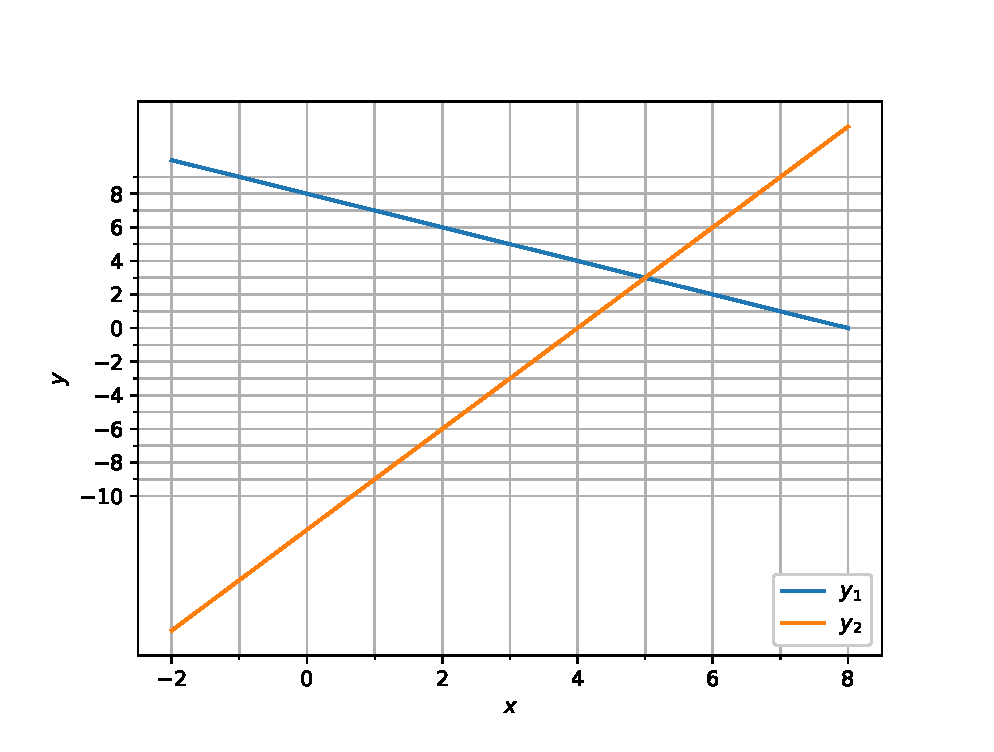
\includegraphics[width=\columnwidth]{./figs/draw_line.eps}
\caption{}
\label{fig:draw_line}
\end{figure}
\item The \textbf{np.linspace} function above generates an arithmetic sequence with first term -2, last term 8 
and 
number of terms 20.  Write your own linspace function and verify.
\\
\solution The code is available below.
\lstinputlisting{./codes/arith_seq.py}
\end{enumerate}
\section{C programming}
\begin{enumerate}[label=\thesection.\arabic*
,ref=\thesection.\theenumi]
\item Write a C program to generate an arithmetic sequence with $t_0 = -2, t_{n-1}= 8, n = 20$ and print it to 
the file \textbf{ap.dat}.
\\
\solution
\lstinputlisting[language=C]{./codes/ap.c}
\item Now execute the following code.
\lstinputlisting{./codes/apdraw.py}
\item Do all computations in Problem \ref{prob:graph} using C and store the data into files.  Import this data 
so that Python is used only for plotting.
\item Write a function for computing the common difference $d$ given $t_0,t_{n-1}$ and $n$.
%\item Write the \textbf{linspace} function in  C. 
\\
\solution
\lstinputlisting[language=C]{./codes/cdfunc.c}

\end{enumerate}
\section{Python  programming exercises}
\begin{enumerate}[label=\thesection.\arabic*
,ref=\thesection.\theenumi]

\item Find $\vec{A}^{-1}$.
\\
\solution  The {\em inverse} of $\vec{A}$ is obtained as
\begin{align}
\label{eq:matrix_inv}
\vec{A}^{-1} &= \frac{1}{\det{\vec{A}}}\myvec{-1 & -1 \\ -3 & 1}
\\
 &= \frac{1}{-4}\myvec{-1 & -1 \\ -3 & 1}
 = \frac{1}{4}\myvec{1 & 1 \\ 3 & -1}
\end{align}
%
\item Write your own function for calculating $\vec{A}^{-1}$
\item Let 
\begin{align}
\label{eq:right_vec}
\vec{c} = \myvec{8 \\12}
\end{align}
Find $\vec{A}^{-1}\vec{b}$
\\
\solution From \eqref{eq:matrix_inv} and \eqref{eq:right_vec},%
\begin{align}
\vec{A}^{-1}\vec{b}&= \frac{1}{4}\myvec{1 & 1 \\ 3 & -1}\myvec{8 \\12}
\\
&= \frac{1}{4}\myvec{1\times8+  1\times12 \\ 3\times8  -1\times12}=\frac{1}{4}\myvec{20 \\12} = \myvec{5 \\3}
\label{eq:sol}
\end{align}
\item Verify that \eqref{eq:sol} is a solution of \eqref{eq:lines}.
\item Write a program to find the solution of \eqref{eq:lines}.
\\
\solution The following program finds the solution 
\lstinputlisting{./codes/eq_sol.py}
\item Write your own program for \textbf{np.matmul}.
\end{enumerate}
\section{C programming exercises}
\begin{enumerate}[label=\thesection.\arabic*
,ref=\thesection.\theenumi]
\item A geometric sequence is defined as
\begin{align}
\label{eq:geo}
t_{n-1} = t_0r^{n-1}
\end{align}
Write a function for generating the $n$th term of a geometric sequence from $t_0, r$ and $n$.
\\
\solution 
\lstinputlisting[language=C]{./codes/gp.c}
%
\item Write a function to calculate simple interest and amount.
\item Write a function to calculate compound interest and amount.
\item Write a function to calculate the circumference of a circle.
\\
\solution 
\lstinputlisting[language=C]{./codes/circum.c}
\item Write a function to calculate the area of a circle.

\item Write a program to find the sum of the first  $n$ terms of an arithmetic sequence. Verify by finding the 
sum of the numbers $1,\dots, 10$.
\\
\solution 
\lstinputlisting[language=C]{./codes/ap_sum.c}
\item Write a program to find the sum of the first  $n$ terms of a geometric sequence.
\item Write a program to check if given lengths  can form the sides of a triangle.
\\
\solution 
\lstinputlisting[language=C]{./codes/tri_side.c}

%\item Write a C program to find $\det\brak{\vec{A}}$.
%\\
%\solution
%\lstinputlisting[language=C]{./codes/det_matrix.c}
\item Write a program to find $\vec{A}^{-1}$ and print it.
\\
\solution 
\lstinputlisting[language=C]{./codes/mat_inv.c}
%\item Write a function to find $\vec{A}^{-1}$.
%\\
%\solution 
%%\lstinputlisting[language=C]{./codes/pointer_matrix_array.c}
\item Write a program to find the intersection of two lines using Cramer's rule.
\item Write a program to verify if two lines intersect.
\item Write a program to find $\vec{A}^{-1}\vec{c}$.
%\\
%\solution 
%\lstinputlisting[language=C]{./codes/pointer_matrix_array.c}

\end{enumerate}

\end{document}


